\documentclass[11pt]{article}
% Revised September 22 and October 7, 2026.
% Compile this standalone source to the corresponding public/pdfs path.
% The revision date is included in the source; no separate stamp is needed.

% ---------- Basic typography and layout ----------
\usepackage[T1]{fontenc}
\usepackage{lmodern}
\usepackage[margin=1in]{geometry}
\usepackage{microtype}
\usepackage{enumitem}
\usepackage{xcolor}

% ---------- Mathematics ----------
\usepackage{amsmath,amssymb,amsthm,mathtools}

% ---------- Diagrams ----------
\usepackage{tikz}
\usetikzlibrary{arrows.meta,calc,decorations.pathreplacing,positioning}

% ---------- Hyperlinks ----------
\usepackage[colorlinks=true,linkcolor=blue!45!black,urlcolor=blue!45!black,citecolor=blue!45!black]{hyperref}
\hypersetup{
  pdftitle={Products Preserve Riemann Integrability: A Local Oscillation Proof},
  pdfauthor={Henry Shin},
  pdfsubject={A local oscillation and Darboux-sum proof of closure under products},
  pdfkeywords={real analysis; Riemann integrability; Darboux sums; oscillation}
}

% ---------- Spacing ----------
\setlength{\parindent}{0pt}
\setlength{\parskip}{0.58em}
\setlist[itemize]{leftmargin=2.2em}
\setlist[enumerate]{leftmargin=2.2em}

% ---------- Macros ----------
\newcommand{\R}{\mathbb{R}}
\newcommand{\dxi}{\Delta x_i}
\DeclareMathOperator{\osc}{osc}

% ---------- Theorem environments ----------
\theoremstyle{plain}
\newtheorem{theorem}{Theorem}
\newtheorem{lemma}{Lemma}
\newtheorem{proposition}{Proposition}

\theoremstyle{remark}
\newtheorem{remark}{Remark}

% ---------- Title ----------
\title{\vspace{-1.4cm}\textbf{Products Preserve Riemann Integrability}\\[0.25em]
\large A Local Oscillation Proof}
\author{Henry Shin}
\date{\small Revised October 7, 2026}

\begin{document}

\maketitle
\vspace{-0.7cm}

\begin{center}
\emph{A proof about boundedness, local variation, and how Darboux estimates are built from pointwise identities.}
\end{center}

\section*{1. Why prove the product theorem this way?}

The theorem is familiar: if $f$ and $g$ are Riemann integrable on a compact interval, then their product $fg$ is Riemann integrable. There are several standard ways to prove this. One can use upper and lower step-function approximations, one can split functions into positive and negative parts, or one can appeal to a more general theorem saying that continuous functions of Riemann integrable functions are Riemann integrable.

The proof below focuses on a local estimate. It asks:
\[
    \textit{If $x$ and $y$ lie in the same small interval, how much can $f(x)g(x)$ differ from $f(y)g(y)$?}
\]

The answer is encoded in the elementary identity
\[
    f(x)g(x)-f(y)g(y)
    =(f(x)-f(y))g(x)+f(y)(g(x)-g(y)).
\]
This identity is the engine of the proof. It separates the motion of the product into two parts: the motion of $f$, multiplied by a bounded value of $g$, and the motion of $g$, multiplied by a bounded value of $f$.

Thus, on every interval $I$, the local oscillation of the product is controlled by the local oscillations of the factors:
\[
    \osc_I(fg)
    \leq
    M_g\,\osc_I(f)+M_f\,\osc_I(g),
\]
where $M_f$ and $M_g$ are global bounds for $|f|$ and $|g|$.

Once this local estimate is known, the Darboux criterion applies: choose a common refinement on which the oscillation sums for $f$ and $g$ are small, and the oscillation sum for $fg$ will be small too.

The point of the note is therefore not just to prove a closure property. The point is to practice a transferable proof pattern:
\[
    \begin{aligned}
    &\text{expand a difference}
    \longrightarrow
    \text{isolate the moving pieces}\\
    &\qquad\longrightarrow
    \text{use boundedness}
    \longrightarrow
    \text{sum local estimates globally}.
    \end{aligned}
\]
This is a flexible analytic maneuver. It avoids sign-splitting and does not rely on multiplication being order-preserving for arbitrary upper and lower approximants. It replaces an order problem with a variation problem.

\section*{2. Darboux notation and oscillation}

Let $u:[a,b]\to\R$ be bounded. If $I\subseteq [a,b]$ is a nonempty subinterval, define the oscillation of $u$ on $I$ by
\[
    \osc_I(u)=\sup_{t\in I}u(t)-\inf_{t\in I}u(t).
\]

Let
\[
    P=\{x_0,x_1,\dots,x_n\},
    \qquad
    a=x_0<x_1<\cdots <x_n=b,
\]
be a partition of $[a,b]$. Write
\[
    I_i=[x_{i-1},x_i],
    \qquad
    \dxi=x_i-x_{i-1}.
\]
Then
\[
    U(P,u)-L(P,u)
    =\sum_{i=1}^n \osc_{I_i}(u)\dxi.
\]

We shall use the Darboux criterion: a bounded function $u$ is Riemann integrable on $[a,b]$ if and only if for every $\varepsilon>0$ there exists a partition $P$ such that
\[
    U(P,u)-L(P,u)<\varepsilon.
\]

The following lemma is a convenient way to estimate oscillations. It lets us replace upper and lower extrema by arbitrary pairs of points.

\begin{lemma}[Oscillation as a two-point supremum]
Let $u:I\to\R$ be bounded on a nonempty interval $I$. Then
\[
    \osc_I(u)=\sup_{x,y\in I}|u(x)-u(y)|.
\]
\end{lemma}

\begin{proof}
Let
\[
    M=\sup_{t\in I}u(t),
    \qquad
    m=\inf_{t\in I}u(t).
\]
For every $x,y\in I$,
\[
    |u(x)-u(y)|\leq M-m,
\]
and therefore
\[
    \sup_{x,y\in I}|u(x)-u(y)|\leq M-m.
\]

Conversely, fix $\eta>0$. By the defining properties of the supremum and infimum, there exist $x,y\in I$ such that
\[
    u(x)>M-\frac{\eta}{2},
    \qquad
    u(y)<m+\frac{\eta}{2}.
\]
Hence
\[
    |u(x)-u(y)|\geq u(x)-u(y)>M-m-\eta.
\]
Since $\eta>0$ was arbitrary,
\[
    \sup_{x,y\in I}|u(x)-u(y)|\geq M-m.
\]
Combining the two inequalities gives
\[
    \osc_I(u)=\sup_{x,y\in I}|u(x)-u(y)|.
\]
\end{proof}

\section*{3. The local product estimate}

The central estimate is purely local. It does not use integrability. It only uses boundedness and the product-difference identity.

\begin{lemma}[Product oscillation estimate]
Let $f,g:I\to\R$ be bounded functions on a nonempty interval $I$. Suppose that
\[
    |f(t)|\leq M_f,
    \qquad
    |g(t)|\leq M_g
\]
for every $t\in I$. Then
\[
    \osc_I(fg)
    \leq
    M_g\,\osc_I(f)+M_f\,\osc_I(g).
\]
\end{lemma}

\begin{proof}
Let $x,y\in I$. We write
\begin{align*}
    f(x)g(x)-f(y)g(y)
    &=f(x)g(x)-f(y)g(x)+f(y)g(x)-f(y)g(y)\\
    &=(f(x)-f(y))g(x)+f(y)(g(x)-g(y)).
\end{align*}
Taking absolute values, and using the bounds on $f$ and $g$, gives
\begin{align*}
    |f(x)g(x)-f(y)g(y)|
    &\leq |f(x)-f(y)|\,|g(x)|+|f(y)|\,|g(x)-g(y)|\\
    &\leq M_g|f(x)-f(y)|+M_f|g(x)-g(y)|.
\end{align*}
Taking the supremum over all $x,y\in I$ and using the preceding lemma, we obtain
\[
    \osc_I(fg)
    \leq
    M_g\,\osc_I(f)+M_f\,\osc_I(g).
\]
\end{proof}

\begin{figure}[h]
\centering
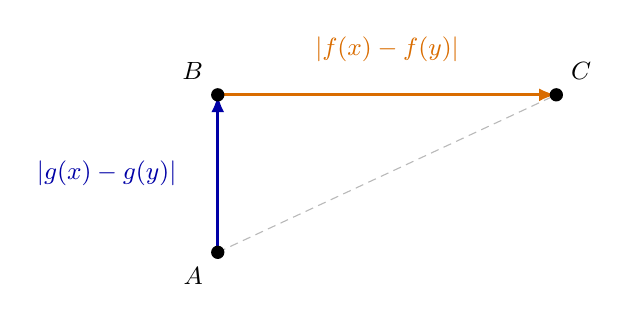
\begin{tikzpicture}[
    >=Latex,
    every node/.style={font=\small},
    point/.style={circle, fill=black, inner sep=1.7pt}
]
    % Schematic only: no axes and no bounded box.
    % The caption supplies the coordinate labels and the boundedness explanation.
    \coordinate (A) at (0,0);
    \coordinate (B) at (0,2.0);
    \coordinate (C) at (4.3,2.0);

    \draw[densely dashed, gray!55] (A) -- (C);

    \draw[very thick, -{Latex[length=2.2mm]}, blue!65!black] (A) -- (B)
        node[midway,left=11pt] {$|g(x)-g(y)|$};
    \draw[very thick, -{Latex[length=2.2mm]}, orange!85!black] (B) -- (C)
        node[midway,above=8pt] {$|f(x)-f(y)|$};

    \node[point,label={below left:$A$}] at (A) {};
    \node[point,label={above left:$B$}] at (B) {};
    \node[point,label={above right:$C$}] at (C) {};
\end{tikzpicture}

\caption{A schematic view of the product-difference identity. Here $A=(f(y),g(y))$, $B=(f(y),g(x))$, and $C=(f(x),g(x))$. Moving from $A$ to $C$ through $B$ first changes the $g$-coordinate and then changes the $f$-coordinate. The vertical move is weighted by $|f(y)|\leq M_f$, and the horizontal move is weighted by $|g(x)|\leq M_g$.}
\end{figure}


\section*{4. Products preserve Riemann integrability}

\begin{theorem}
Let $a<b$, and let $f,g:[a,b]\to\R$ be Riemann integrable functions. Then $fg$ is Riemann integrable on $[a,b]$.
\end{theorem}

\begin{proof}
Since Riemann integrable functions on compact intervals are bounded, choose constants $M_f,M_g>0$ such that
\[
    |f(x)|\leq M_f,
    \qquad
    |g(x)|\leq M_g
\]
for every $x\in [a,b]$.

Fix $\varepsilon>0$. Choose
\[
    \rho=\frac{\varepsilon}{M_f+M_g+1}.
\]
Since $f$ and $g$ are Riemann integrable, there exist partitions $P_1$ and $P_2$ of $[a,b]$ such that
\[
    U(P_1,f)-L(P_1,f)<\rho
\]
and
\[
    U(P_2,g)-L(P_2,g)<\rho.
\]
Let
\[
    P=P_1\cup P_2=\{x_0,x_1,\dots,x_n\},
    \qquad
    a=x_0<x_1<\cdots <x_n=b.
\]
Because refinement decreases the difference between the upper and lower Darboux sums, we have
\[
    U(P,f)-L(P,f)<\rho,
    \qquad
    U(P,g)-L(P,g)<\rho.
\]

For each $i$, write
\[
    I_i=[x_{i-1},x_i],
    \qquad
    \dxi=x_i-x_{i-1}.
\]
By the product oscillation estimate,
\[
    \osc_{I_i}(fg)
    \leq
    M_g\,\osc_{I_i}(f)+M_f\,\osc_{I_i}(g).
\]
Multiplying by $\dxi$ and summing gives
\begin{align*}
    U(P,fg)-L(P,fg)
    &=\sum_{i=1}^n \osc_{I_i}(fg)\dxi\\
    &\leq
    M_g\sum_{i=1}^n \osc_{I_i}(f)\dxi
    +M_f\sum_{i=1}^n \osc_{I_i}(g)\dxi\\
    &=M_g\bigl(U(P,f)-L(P,f)\bigr)
    +M_f\bigl(U(P,g)-L(P,g)\bigr)\\
    &<M_g\rho+M_f\rho\\
    &=(M_f+M_g)\rho\\
    &<\varepsilon.
\end{align*}
Therefore, for every $\varepsilon>0$, there exists a partition $P$ such that
\[
    U(P,fg)-L(P,fg)<\varepsilon.
\]
By the Darboux criterion, $fg$ is Riemann integrable on $[a,b]$.
\end{proof}

\section*{5. From local oscillation to Darboux sums}

The entire proof is organized around the estimate
\[
    \boxed{\;
    \osc_I(fg)
    \leq
    M_g\,\osc_I(f)+M_f\,\osc_I(g)
    \;}
\]
for every nonempty subinterval $I\subseteq [a,b]$.

This estimate converts local information about $f$ and $g$ into local information about $fg$. Once we multiply by interval lengths and sum, the local estimate becomes a Darboux estimate:
\[
    U(P,fg)-L(P,fg)
    \leq
    M_g\bigl(U(P,f)-L(P,f)\bigr)
    +M_f\bigl(U(P,g)-L(P,g)\bigr).
\]
The argument proceeds as follows:

\begin{center}
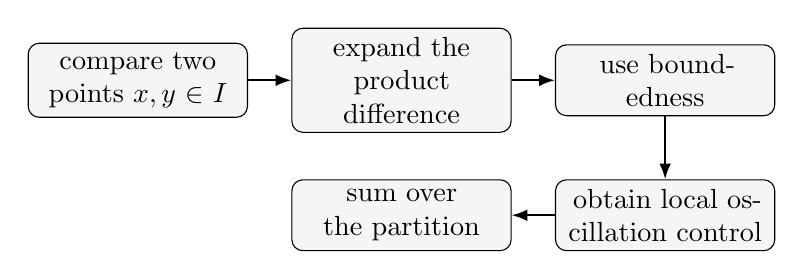
\begin{tikzpicture}[
    flowstep/.style={draw, rounded corners, fill=gray!8, align=center, minimum height=0.9cm, text width=2.55cm},
    arr/.style={-{Latex[length=2mm]}, thick}
]
    \node[flowstep] (s1) {compare two points $x,y\in I$};
    \node[flowstep, right=0.55cm of s1] (s2) {expand the product difference};
    \node[flowstep, right=0.55cm of s2] (s3) {use boundedness};
    \node[flowstep, below=0.8cm of s3] (s4) {obtain local oscillation control};
    \node[flowstep, left=0.55cm of s4] (s5) {sum over the partition};

    \draw[arr] (s1) -- (s2);
    \draw[arr] (s2) -- (s3);
    \draw[arr] (s3) -- (s4);
    \draw[arr] (s4) -- (s5);
\end{tikzpicture}
\end{center}

\section*{6. Why this avoids sign-splitting}

There is a subtle reason some upper/lower approximation proofs of the product theorem become longer than one might expect. If
\[
    \underline f\leq f\leq \overline f,
    \qquad
    \underline g\leq g\leq \overline g,
\]
it is not generally true that
\[
    \underline f\,\underline g\leq fg\leq \overline f\,\overline g.
\]
Multiplication is monotone in each variable only under sign restrictions. This is why one often splits into positive and negative parts before multiplying minorants and majorants.

The oscillation proof bypasses that issue. It does not ask whether products of minorants minorize or products of majorants majorize. It asks instead:
\[
    \textit{How far apart can two values of the product be on the same small interval?}
\]
This question is answered directly by
\[
    f(x)g(x)-f(y)g(y)
    =(f(x)-f(y))g(x)+f(y)(g(x)-g(y)).
\]
No positivity is required. The possible sign changes of $f$ and $g$ are absorbed by absolute values and boundedness.

The estimate therefore controls variation without imposing sign restrictions.

\section*{7. Other Lipschitz constructions}

Let $f_1,\ldots,f_m:[a,b]\to\R$ be Riemann integrable, and suppose $F:\R^m\to\R$ is Lipschitz on a bounded set containing their joint range. Put $h(x)=F(f_1(x),\ldots,f_m(x))$. The function $h$ is bounded, and for some constant $C\geq0$,
\begin{align*}
&\left|F(f_1(x),\dots,f_m(x))-F(f_1(y),\dots,f_m(y))\right|\\
&\qquad\leq C\left(|f_1(x)-f_1(y)|+\cdots+|f_m(x)-f_m(y)|\right)
\end{align*}
Taking suprema over $x,y$ in a nonempty subinterval $I$ gives
\[
    \osc_I(h)\leq C\sum_{j=1}^m\osc_I(f_j).
\]
Multiplying by interval lengths and summing gives the corresponding bound for the Darboux gaps. A common refinement makes the gaps for all $f_j$ simultaneously small, proving that $h$ is Riemann integrable.

For multiplication, $F(s,t)=st$ is not globally Lipschitz on all of $\R^2$, but it is Lipschitz on every bounded rectangle. Since Riemann integrable functions on compact intervals are bounded, this is enough.

For maximum, $F(s,t)=\max(s,t)$ is globally Lipschitz, and the same estimate gives
\[
    \osc_I(\max(f,g))
    \leq
    \osc_I(f)+\osc_I(g).
\]

\end{document}
